\subsection{Casos de Teste}\label{sec:testes}
Nessa seção demostraremos alguns exemplos de casos de teste do problema Tutores e qual o comportamento da \textit{Splay Tree} ao realizar a inserção das matrículas.

\subsubsection{Exemplo de Caso de Teste 1}
\begin{lstlisting}[frame=single,caption=Instância de teste 1,label=test1,escapeinside={\%*}{*)},inputencoding=utf8]
  3     // %*Número de estudantes*)
  5 1 2 // %*Ordem de inserção dos estudantes*)
  1     // %*Quantas consultas serão realizadas*)
  2     // %*Tutor do estudante 2*)
\end{lstlisting}

\begin{figure}[htb]
\centering
% dot -Gdpi=300 -Tpng test1.dot > test1.png
%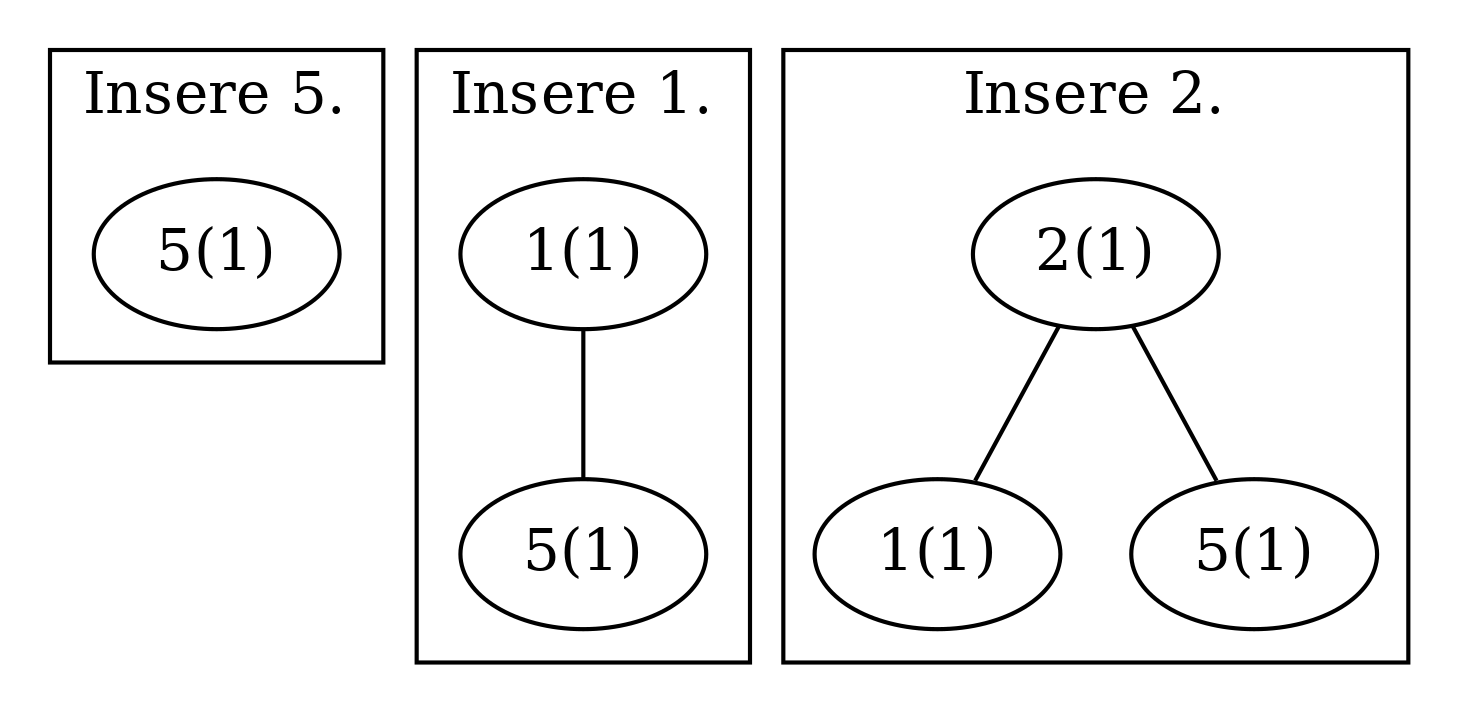
\includegraphics[width=0.5\linewidth]{test1.png}
\begin{forest}
[5
	[$\emptyset$]
	[$\emptyset$]
]
\end{forest}
\hspace{1em}
\begin{forest}
[1
	[$\emptyset$]
	[5
		[$\emptyset$]
		[$\emptyset$]
	]
]
\end{forest}
\hspace{1em}
\begin{forest}
[2
	[1
		[$\emptyset$]
		[$\emptyset$]
	]
	[5
		[$\emptyset$]
		[$\emptyset$]
	]
]
\end{forest}
\caption{\textit{Splay Tree} após cada inserção de chave do Caso de Teste 1}
\label{fig:test1}
\end{figure}

\subsubsection{Exemplo de Caso de Teste 2}
\begin{lstlisting}[frame=single,caption=Instância de teste 1,label=test2,escapeinside={\%*}{*)},inputencoding=utf8]
  5         // %*Número de estudantes*)
  3 1 4 2 5 // %*Ordem de inserção dos estudantes*)
  2         // %*Quantas consultas serão realizadas*)
  2 5       // %*Tutores dos estudantes 2 e 5*)
\end{lstlisting}

\begin{figure}[htb]
\centering
% dot -Gdpi=300 -Tpng test2.dot > test2.png
%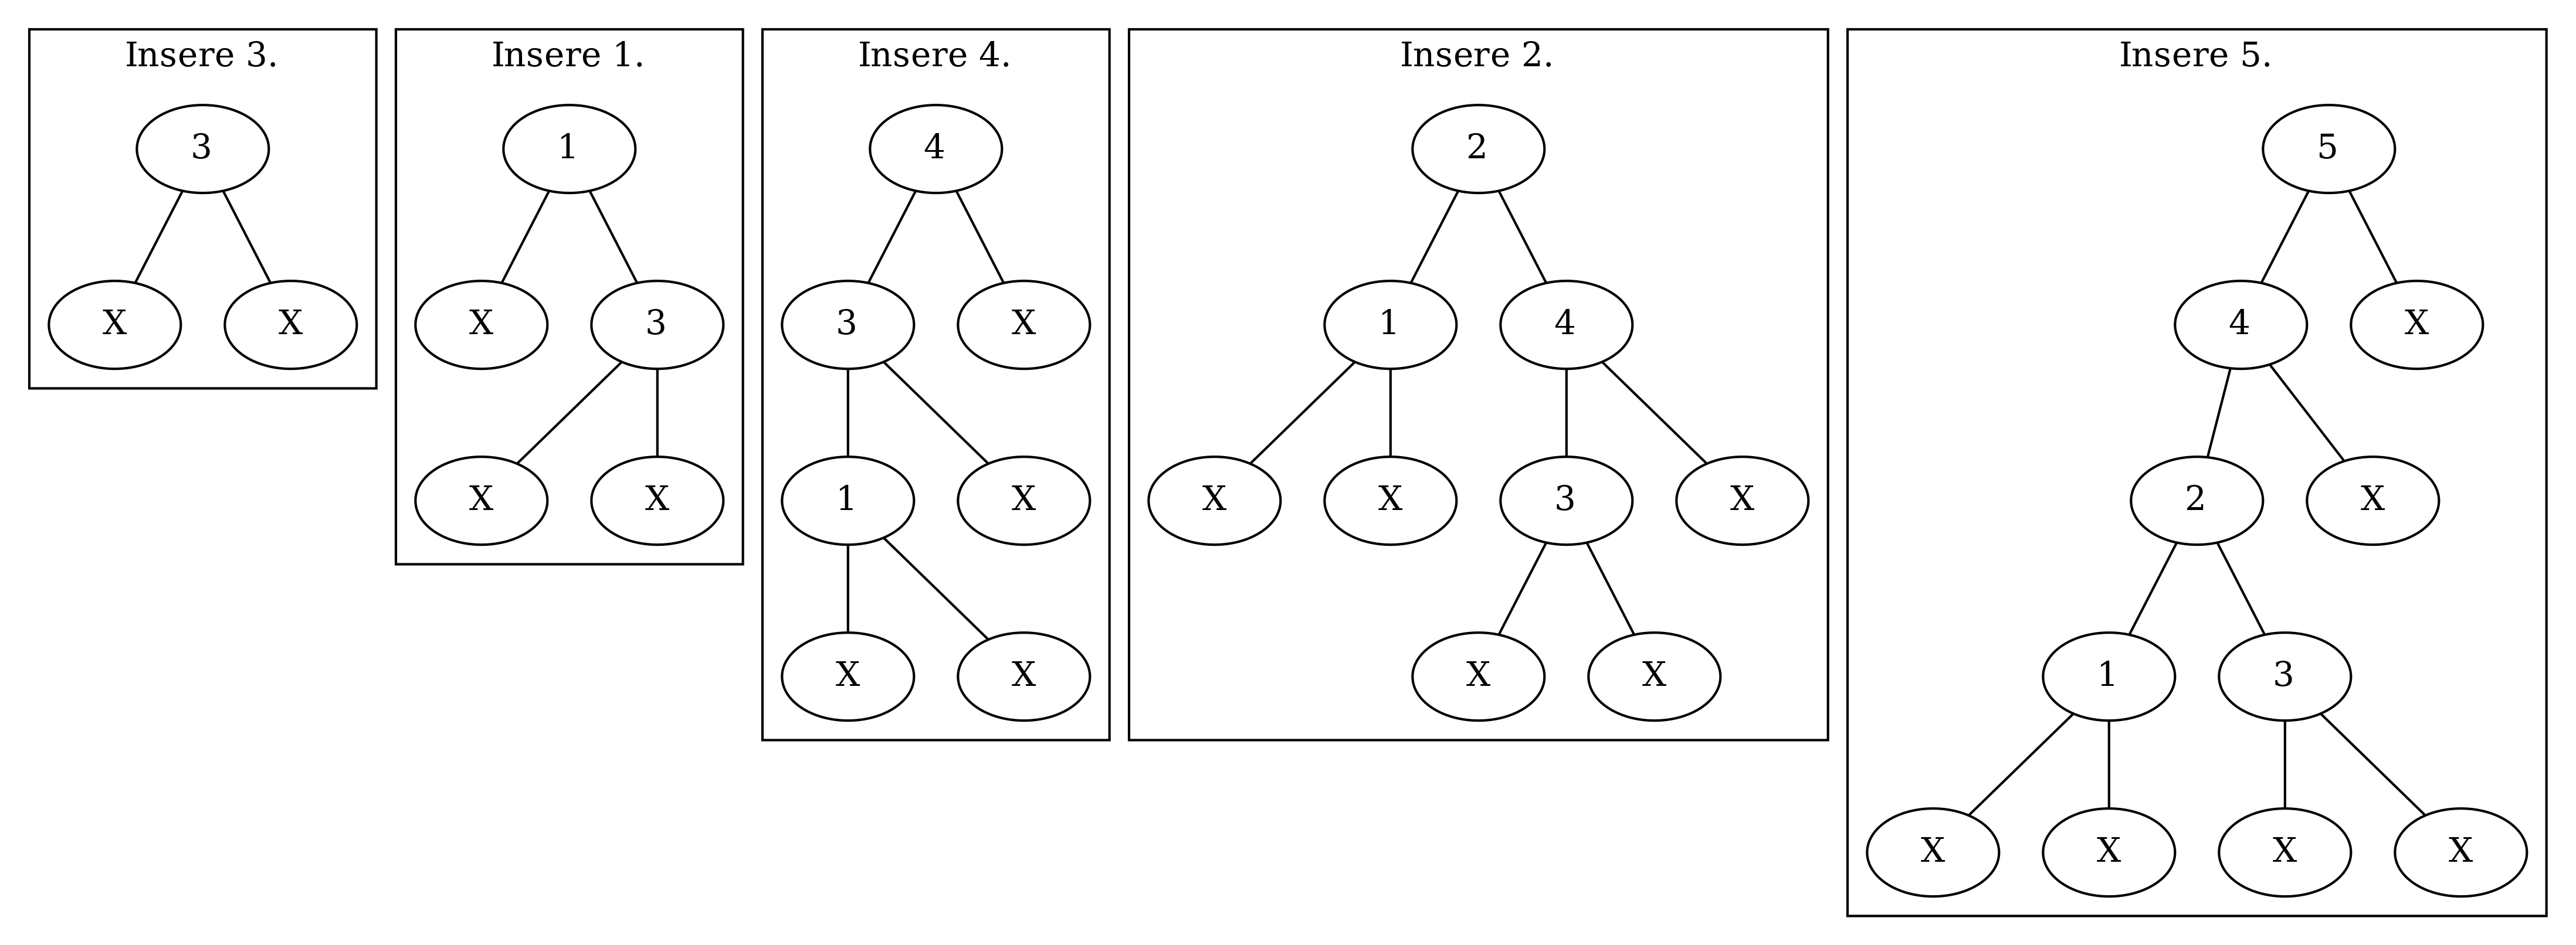
\includegraphics[width=\linewidth]{test2.png}
\begin{forest}
[3
	[$\emptyset$]
	[$\emptyset$]
]
\end{forest}
\hspace{1em}
\begin{forest}
[1
	[$\emptyset$]
	[3
		[$\emptyset$]
		[$\emptyset$]
	]
]
\end{forest}
\hspace{1em}
\begin{forest}
[4
	[3
		[1
			[$\emptyset$]
			[$\emptyset$]
		]
		[$\emptyset$]
	]
	[$\emptyset$]
]
\end{forest}
\hspace{1em}
\begin{forest}
[2
	[1
		[$\emptyset$]
		[$\emptyset$]
	]
	[4
		[3
			[$\emptyset$]
			[$\emptyset$]
		]
		[$\emptyset$]
	]
]
\end{forest}
\hspace{1em}
\begin{forest}
[5
	[4
		[2
			[1
				[$\emptyset$]
				[$\emptyset$]
			]
			[3
				[$\emptyset$]
				[$\emptyset$]
			]
		]
		[$\emptyset$]
	]
	[$\emptyset$]
]
\end{forest}
\caption{\textit{Splay Tree} após cada inserção de chave do Caso de Teste 2}
\label{fig:test2}
\end{figure}

\subsubsection{\textit{Benchmarks}}
Com o objetivo de verificar o tempo de execução, testamos nossa solução com casos de diferentes de tamanhos. São dois tipos de casos em tamanhos de $10$ à $10^5$ com as chaves gerados uniformemente aleatórias:
\begin{itemize}
\item Matrículas em qualquer ordem (não ordenadas).
\item Matrículas \textbf{ordenadas}.
\end{itemize}

Os tempos de execução estão descrito no gráfico da figura \ref{fig:benchmark}.

\begin{figure}[!ht]
\centering
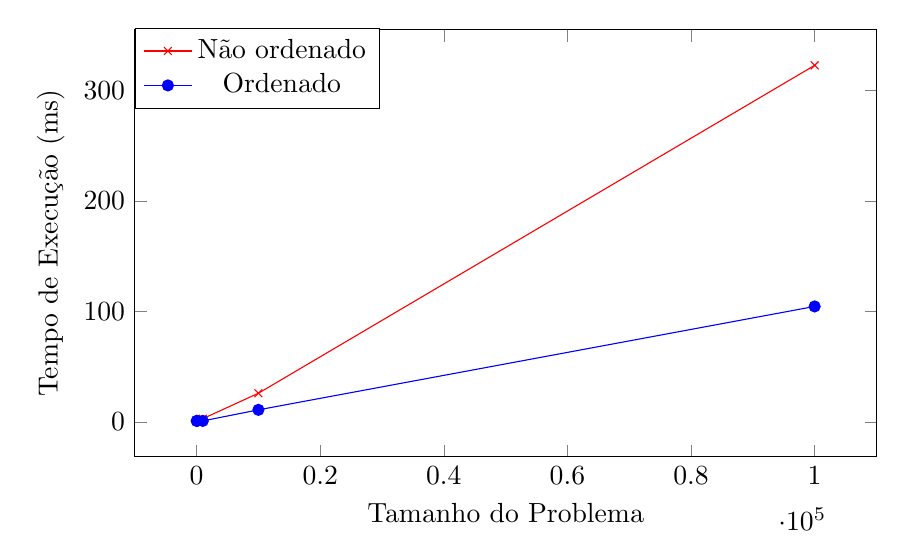
\begin{tikzpicture}[]
\begin{axis}[
	xlabel=Tamanho do Problema,
	ylabel=Tempo de Execução (ms),
	width=11cm,height=7cm,
    legend style={at={(0.0,.91)},anchor=west}
    ]

\addplot[color=red,mark=x] coordinates {
(10, 1)
(100, 1)
(1000, 3)
(10000, 26)
(100000, 322.5)
};

\addplot[color=blue,mark=*] coordinates {
(10, 1)
(100, 1)
(1000, 1)
(10000, 11)
(100000, 104.5)
};

\legend{Não ordenado, Ordenado}
\end{axis}
\end{tikzpicture}
\caption{Tempo de execução em milissegundos para os testes gerados.}
\label{fig:benchmark}
\end{figure}

Se observa um tempo melhor para os casos em que as chaves são adicionadas em \textbf{ordem crescente}, o que pode ser explicado pois a cada inserção o último nó inserido vai estar na raiz da \textit{Splay Tree} (por característica da estrutura de dados) e como esse nó vai ser o pai do nó que está sendo inserido nesse momento, isso acelera a busca por ele.
